\section{Experiments}\label{sec:experiments}

\subsection{Experimental Setup}\label{sec:setup}

\paragraph{Datasets.}
We evaluate on four English NER benchmarks spanning a difficulty gradient.
\textbf{SciERC} \cite{luan2018scierc} (551 test instances, 6 entity types) is the primary medium-difficulty test bed (${\approx}$65\% F1).
\textbf{Few-NERD} \cite{ding2021fewnerd} (INTRA coarse; 37{,}648 instances, 8 entity types, ${\approx}$75\% F1) provides a low-degeneracy contrast where LP selection succeeds (\S\ref{sec:selection_gap}).
\textbf{CoNLL-2003} \cite{tjongkimsang2003conll} (3{,}453 test sentences, 4 entity types, ${\approx}$91\% F1) serves as a ceiling-effect control.
\textbf{WNUT-17} \cite{derczynski2017wnut} (1{,}287 social media instances, 53.7\% zero F1) probes the signal-collapse boundary.

\paragraph{Models and sampling.}
\textbf{Qwen3-8B} and \textbf{LLaMA-3.1-8B-Instruct} are LoRA fine-tuned using LLaMA Factory \cite{zheng2024llamafactory} (Appendix~\ref{app:training}; Few-NERD uses 3 epochs vs.\ 5 for others; Appendix~\ref{app:epoch_confound}).
$N{=}8$ samples at $T{=}1.0$ (primary) with vLLM constrained decoding \cite{willard2023guided}; $N {\in} \{16, 32, 64\}$ for scaling (Figure~\ref{fig:n_scaling}; Appendix~\ref{app:n_scaling}).

\begin{figure}[t]
\centering
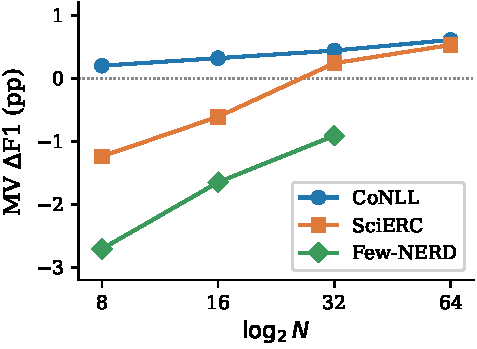
\includegraphics[width=\columnwidth]{figures/fig_n_scaling_mv.pdf}
\caption{MV $\Delta$F1 vs.\ $\log_2 N$ across three datasets (Qwen3-8B FT, seed${=}42$). Dotted gray: $\Delta{=}0$. Gains are dataset-dependent: persistently negative on Few-NERD, near zero on SciERC at higher $N$, marginally positive on CoNLL ($+0.6$\,pp at $N{=}64$).}
\label{fig:n_scaling}
\end{figure}

%% ============================================================
\subsection{Quality Estimation Results}\label{sec:qe_results}

\begin{table*}[t]
\centering
\small
\caption{NER quality estimation ($\rho$ and AUROC; $N{=}8$, primary seed${=}42$; 5-seed $\sigma{\leq}0.026$ in Table~\ref{tab:multiseed}). AUROC binarizes at per-dataset median F1. Best in \textbf{bold}. RE in Appendix~\ref{app:re_extension}; $N{=}16$ in Table~\ref{tab:robustness}.}
\label{tab:quality_estimation}
\begin{tabular}{ll cc cc cc}
\toprule
& & \multicolumn{2}{c}{\textbf{SciERC}} & \multicolumn{2}{c}{\textbf{CoNLL (Qwen)}} & \multicolumn{2}{c}{\textbf{CoNLL (LLaMA)}} \\
\cmidrule(lr){3-4} \cmidrule(lr){5-6} \cmidrule(lr){7-8}
Signal & Family & $\rho$ & AUC & $\rho$ & AUC & $\rho$ & AUC \\
\midrule
VC & Structural & \textbf{.379} & .684 & .424 & .789 & .426 & .709 \\
SJ  & Structural & .360 & \textbf{.692} & .436 & .801 & \textbf{.431} & .704 \\
FK & Surface & .267 & .629 & .400 & .774 & .428 & .703 \\
EM  & Surface    & .295 & .631 & \textbf{.451} & \textbf{.816} & \textbf{.431} & .705 \\
\midrule
LP     & Model      & .205 & .578 & .316 & .753 & .307 & \textbf{.761} \\
\bottomrule
\end{tabular}
\end{table*}

Table~\ref{tab:quality_estimation} presents $\rho$ and AUROC for five signals across tasks and models.

\paragraph{Signal rankings are difficulty-dependent.}
On SciERC, structural signals lead (VC $\rho{=}0.379$, SJ $0.360$) over LP ($0.205$); bootstrap CIs confirm the gap ($\Delta\rho{=}{+}0.151{\pm}0.006$, 5 seeds; Appendix~\ref{app:bootstrap_signal}).
Under seed-replication Holm--Bonferroni correction ($k{=}5$ seeds), the SJ~${>}$~LP advantage reaches $p_{\text{adj}}{=}0.013$ (Appendix~\ref{app:bootstrap_signal}).
On CoNLL (F1${\approx}$0.91), EM leads both $\rho$ and AUROC ($0.816$).
At the signal-collapse boundary (WNUT-17, F1${\approx}$42\%), full-set correlations are dominated by the zero/non-zero boundary (VC $\rho{=}0.724$ at $N{=}16$, but conditional $\rho{=}0.038$; Table~\ref{tab:wnut}); LP shows the reverse (conditional $\rho{=}0.350$; Figure~\ref{fig:signal_heatmap}).

%% ============================================================
\subsection{Cross-Dataset Contrast: Few-NERD}\label{sec:fewnerd}

\begin{table}[t]
\centering
\small
\caption{LP selection across datasets (instance-averaged F1; Qwen3-8B, $N{=}8$, $T{=}1.0$, gold-filtered, 3-seed means). $p$: paired bootstrap.}
\label{tab:fewnerd}
\resizebox{\columnwidth}{!}{%
\begin{tabular}{@{}lrccccr@{}}
\toprule
Dataset & $n$ & Greedy & Degen.\% & LP $\rho$ & LP $\Delta$ & $p$ \\
\midrule
WNUT-17 & 1{,}287 & .452 & 67.9\% & $-$.446 & $-$0.45\,pp & .72 \\
CoNLL & 2{,}756 & .908 & 61.7\% & .302 & $-$0.85\,pp & 1.0 \\
SciERC & 529 & .663 & 12.2\% & .159 & $+$0.61\,pp & .193 \\
Few-NERD & 32{,}565 & .748 & 13.0\% & .220 & $\mathbf{+1.39}$\,pp & ${<}.001$ \\
\bottomrule
\end{tabular}}
\end{table}

Few-NERD (Table~\ref{tab:fewnerd}) confirms LP selection at low degeneracy ($+1.39$~pp\footnote{Under corpus micro-F1, LP $\Delta{=}+0.09{\pm}0.03$\,pp; the larger instance-averaged gains concentrate on few-entity instances.}, $p{<}0.001$; structural signals degrade: VC $-1.79$, SJ $-2.14$~pp), with LP 50$\times$ more seed-stable ($\sigma{=}0.04$ vs.\ SJ $2.02$~pp), generalizing to LLaMA (Table~\ref{tab:cross_selection}). Training convergence modulates degeneracy (5-epoch: $26$\%, LP $\Delta$ collapses from $+1.39$ to $+0.12$\,pp; Appendix~\ref{app:epoch_confound}).

Signal ranking is task-specific; per-type analysis shows MV degradation concentrates in low-F1 types ($\rho{=}0.90$, $p{=}0.002$; Appendix~\ref{app:pertype}).

\paragraph{Degeneracy alone does not predict LP direction.}
Degeneracy does not predict LP gain across 23 configurations ($\rho{=}0.052$, $p{=}0.81$; $n{=}23$, insufficient for reliable correlation---we treat this as supplementary evidence; Figure~\ref{fig:degeneracy_scatter}), though it co-varies with LP within fixed settings ($\rho{=}{-}0.881$; Appendix~\ref{app:per_type_lp}).

\begin{figure}[t]
\centering
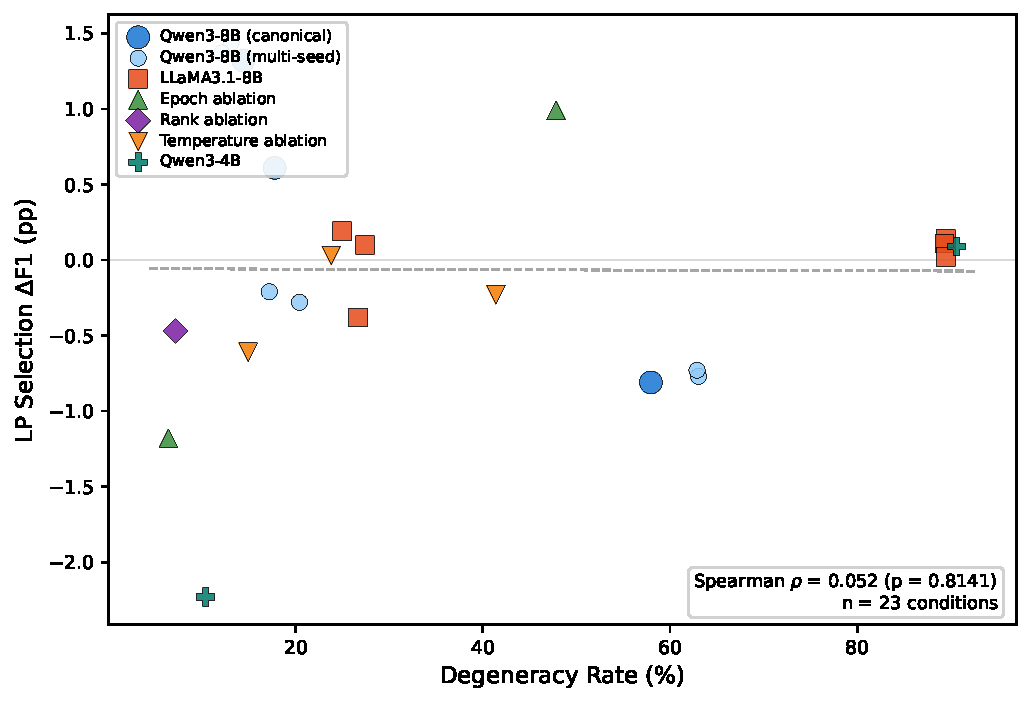
\includegraphics[width=\columnwidth]{figures/fig_degeneracy_lp_scatter.pdf}
\caption{Instance degeneracy vs.\ LP selection gain across 23 configurations ($N{=}8$; $\rho{=}0.052$, $p{=}0.81$). Within Few-NERD per-entity-type ($\rho{=}{-}0.881$; Appendix~\ref{app:per_type_lp}), degeneracy predicts LP gain when alignment is held constant.}
\label{fig:degeneracy_scatter}
\end{figure}

MV gains range from $-2.71$\,pp (Few-NERD) to $+0.6$\,pp (CoNLL at $N{=}64$; Figure~\ref{fig:n_scaling}); the optimal strategy is dataset-dependent (LP-best $+1.4$\,pp on Few-NERD vs.\ MV $+0.6$\,pp on CoNLL).
The framework extends to RE, where $40$\% zero-F1 from upstream entity span errors creates a distinct failure mode---\textit{diversity among failures} rather than quality-differentiated outputs---despite comparable degeneracy ($10.1$\% vs.\ SciERC NER $12.2$\%; Appendix~\ref{app:re_extension}).

%% ============================================================
\subsection{Robustness}\label{sec:robustness_main}

Signal rankings are robust across temperatures, seeds, and $N$ (Table~\ref{tab:robustness}; Appendix~\ref{app:calibration}); Qwen3-4B QE matches 8B ($|\Delta\rho|{=}0.042$).
The gap persists from 4B to 72B zero-shot to GPT-5.5 (\S\ref{sec:scaling}).

%% ============================================================
\subsection{Entity Construction (Exploratory)}\label{sec:prescriptive}

\paragraph{Entity-level construction.}
We aggregate entities across samples, retaining those exceeding $\theta{=}2/N$ with LP-weighted scoring ($\theta$ stable in $[0.15, 0.35]$; Appendix~\ref{app:theta_sweep}).
LP-weighted construction yields $+1.40{\pm}0.51$\,pp on Few-NERD (4-seed mean; $p{<}0.001$; Table~\ref{tab:entity_construction}), consistent with favorable diagnostic conditions ($D{=}13$\%, headroom${=}12.4$\,pp), a non-significant $+0.32$\,pp on SciERC, and no gain on CoNLL ($-0.39$\,pp).\footnote{Degenerate instances contribute $\Delta{=}0$ by construction; all gains concentrate in the non-degenerate subset.}
Under per-family Holm--Bonferroni \cite{holm1979simple} correction ($k{=}10$ entity-construction comparisons), $p_{\text{adj}}{=}0.006$; global ($k{=}57$): $p_{\text{adj}}{=}0.055$; the family partition was not pre-registered (Appendix~\ref{app:holm}).
Construction and LP selection are complementary ($\rho_{\text{adj}}$: Few-NERD $0.516$; Table~\ref{tab:cross_selection}).
Training convergence modulates returns: 5-epoch Few-NERD eliminates LP gains (selection: $+1.39{\to}+0.12$\,pp; construction: $+0.88{\to}+0.20$\,pp) as degeneracy rises from $9$\% to $26$\% (Appendix~\ref{app:epoch_confound}).

\phantomsection\label{sec:selection_results}

\paragraph{Discussion and conclusion.}\label{sec:discussion}\label{sec:selection_method}\label{sec:conclusion}
For discrete-answer reasoning, sample diversity reflects diverse reasoning paths; for NER, degeneracy ($12$--$68$\%) reduces candidate diversity while signal alignment collapse ($\alpha{\to}0$) limits ranking.
The degeneracy decomposition (\S\ref{sec:theory}) identifies $\alpha$---not degeneracy---as the binding constraint ($8$--$33{\times}$ tighter); this persists across families \cite{yun2025price}, scales (4B--72B), and decoding modes (Appendix~\ref{app:freeform_ablation}).
The diagnostic framework---identifying these co-occurring conditions---is our primary contribution; pretrained Qwen2.5-7B at $N{=}32$ achieves $+3.85$\,pp MV gain where the framework predicts favorable conditions ($D{=}5.4$\%; Appendix~\ref{app:n_scaling}).
At $N{=}8$, high degeneracy ($>50$\%) suggests scaling will not help; low degeneracy with strong LP-F1 alignment may warrant exploratory entity construction; otherwise, greedy decoding remains the default.
